\chapter{DEEP LEARNING METHODS}\label{deep_methods}

As with many different computer vision problems, deep learning methods have been used for image inpainting.
The reason why deep learning methods are being used more frequently as time progresses is that they provide more successful results in complex problems compared to traditional methods. The main reason for this is the creation of large-scale datasets that will enable the training of deep methods and the computational power that allow the training of these deep methods.

\section{CNN-based Methods}

Convolutional neural network structures, which are known to be very successful in computer vision studies thanks to their grid-like layer topology, are also used in image inpainting studies and give outstanding results. There are many architectures specially designed for inpainting work.

\begin{figure}[h]
    \centering
    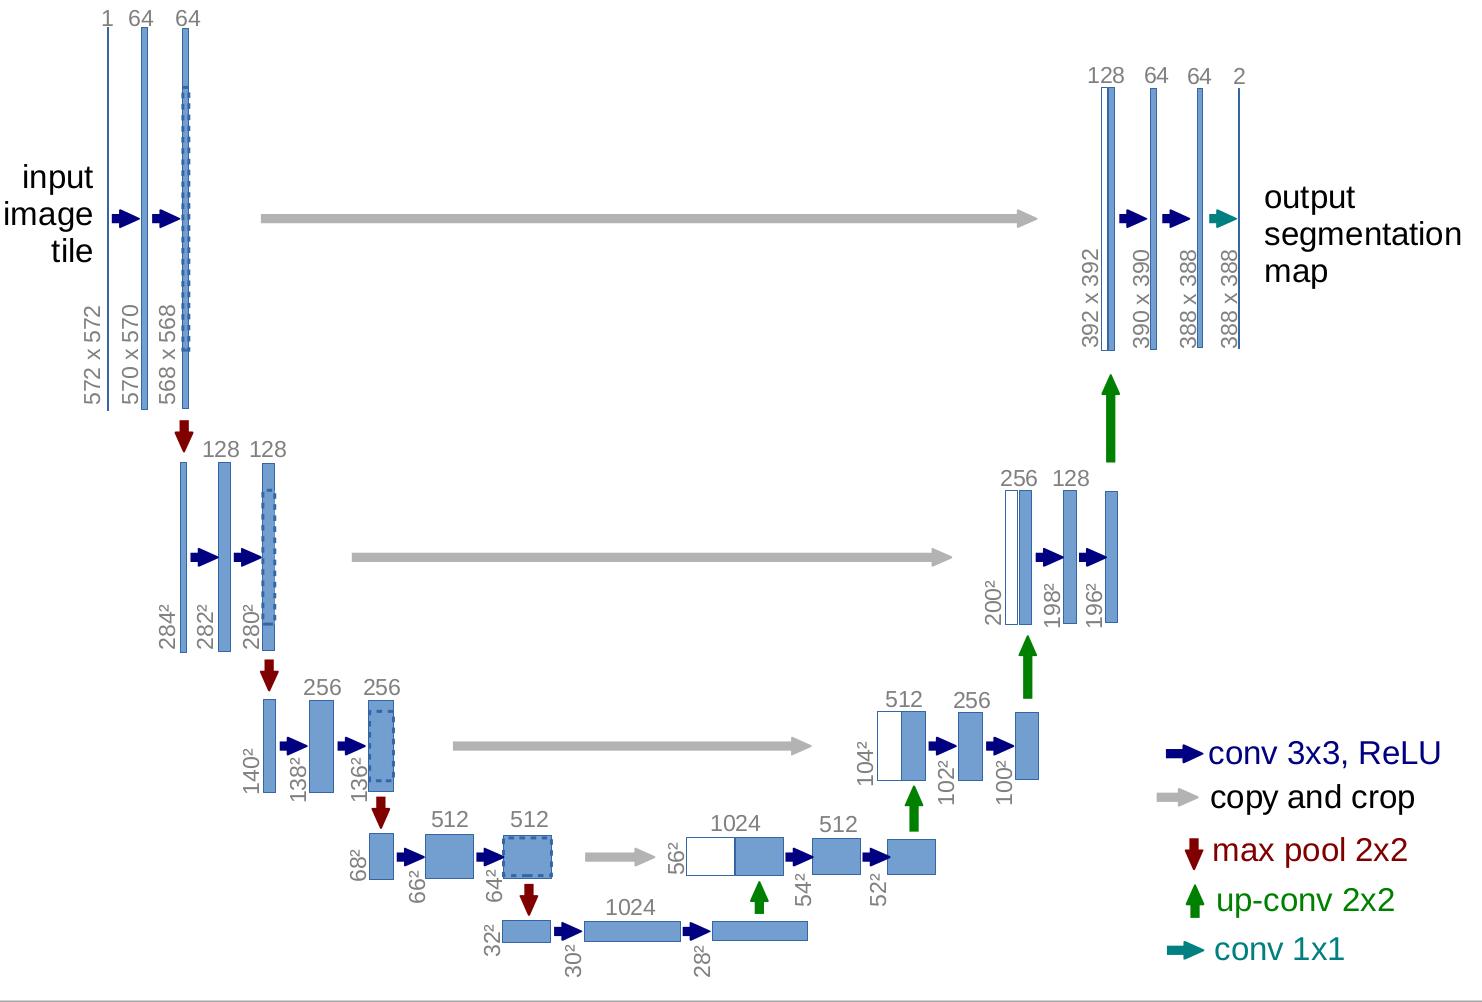
\includegraphics[width=10cm]{figures/chapter4/unet.png}
    \vspace*{5mm}
    \caption{U-Net Architecture \cite{unet}}
    \label{fig:u-net}
\end{figure}

The U-Net \cite{unet} architecture used in Shift-Net inpainting study \cite{shiftNet} is one of them. The U-Net CNN architecture is shown in figure \ref{fig:u-net}  This architecture takes an image and a mask which shows the missing areas and put them into convolutional layers. It concatenate the output of each layer with the corresponding layer of the same size in symmetrical architecture. The results of this structure achieve excellent success in terms of genereted image structure and fine detail. The architecture of the Shift-Net which is a U-Net with special shift-connections can be seen in figure \ref{fig:shiftNet}

\begin{figure}[h]
    \centering
    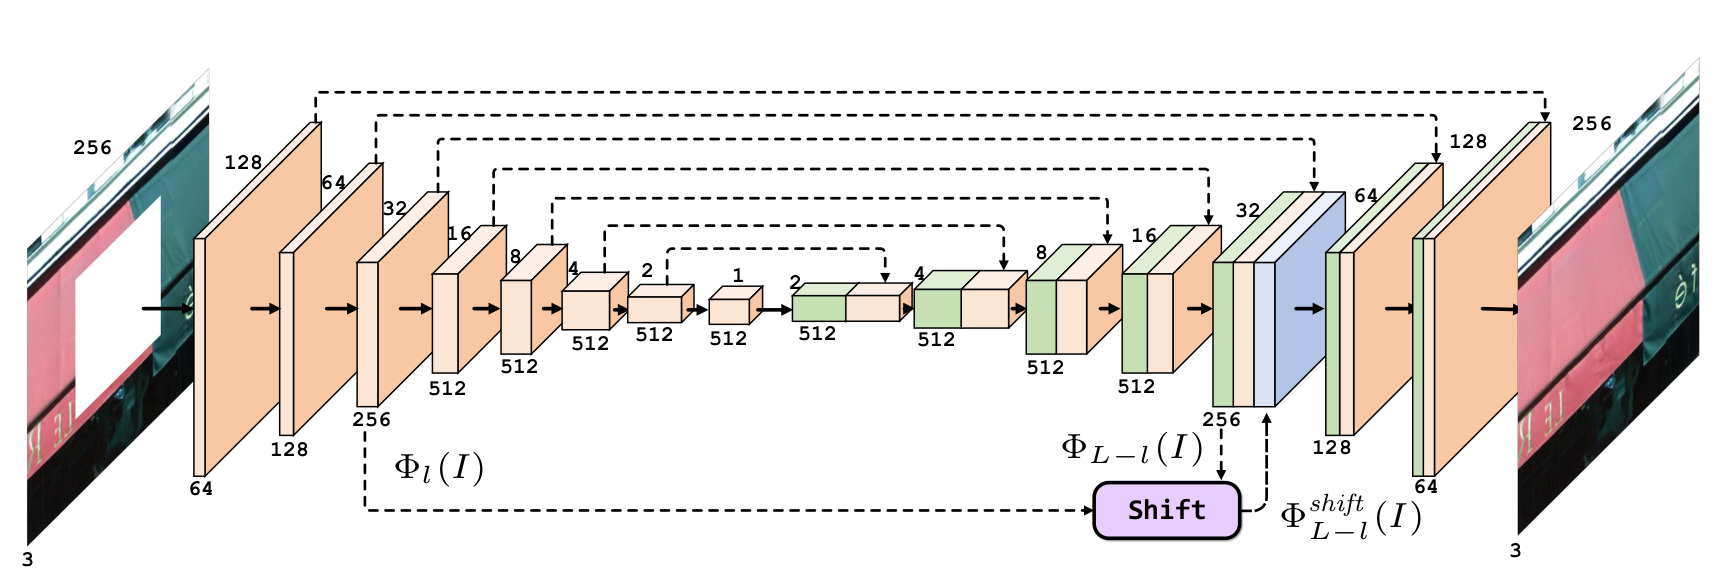
\includegraphics[width=13cm]{figures/chapter4/shiftnet.png}
    \vspace*{5mm}
    \caption{Shift-Net Architecture \cite{shiftNet}}
    \label{fig:shiftNet}
\end{figure}

Another popular architecture used in inpainting studies is the encoder-decoder network. Sidorov and Hardeberg \cite{3DCNN} uses a 3D CNN encoder-decoder network architecture and can perform not only inpainting but also tasks such as denoising and super-resolution. In the study of Liu et al. \cite{csa_layer} coherent semantic attention layer designed and used in an encoder-decoder structure called refinement network. This architecture can be seen in figure \ref{fig:csa_layer}.

\begin{figure}[h]
    \centering
    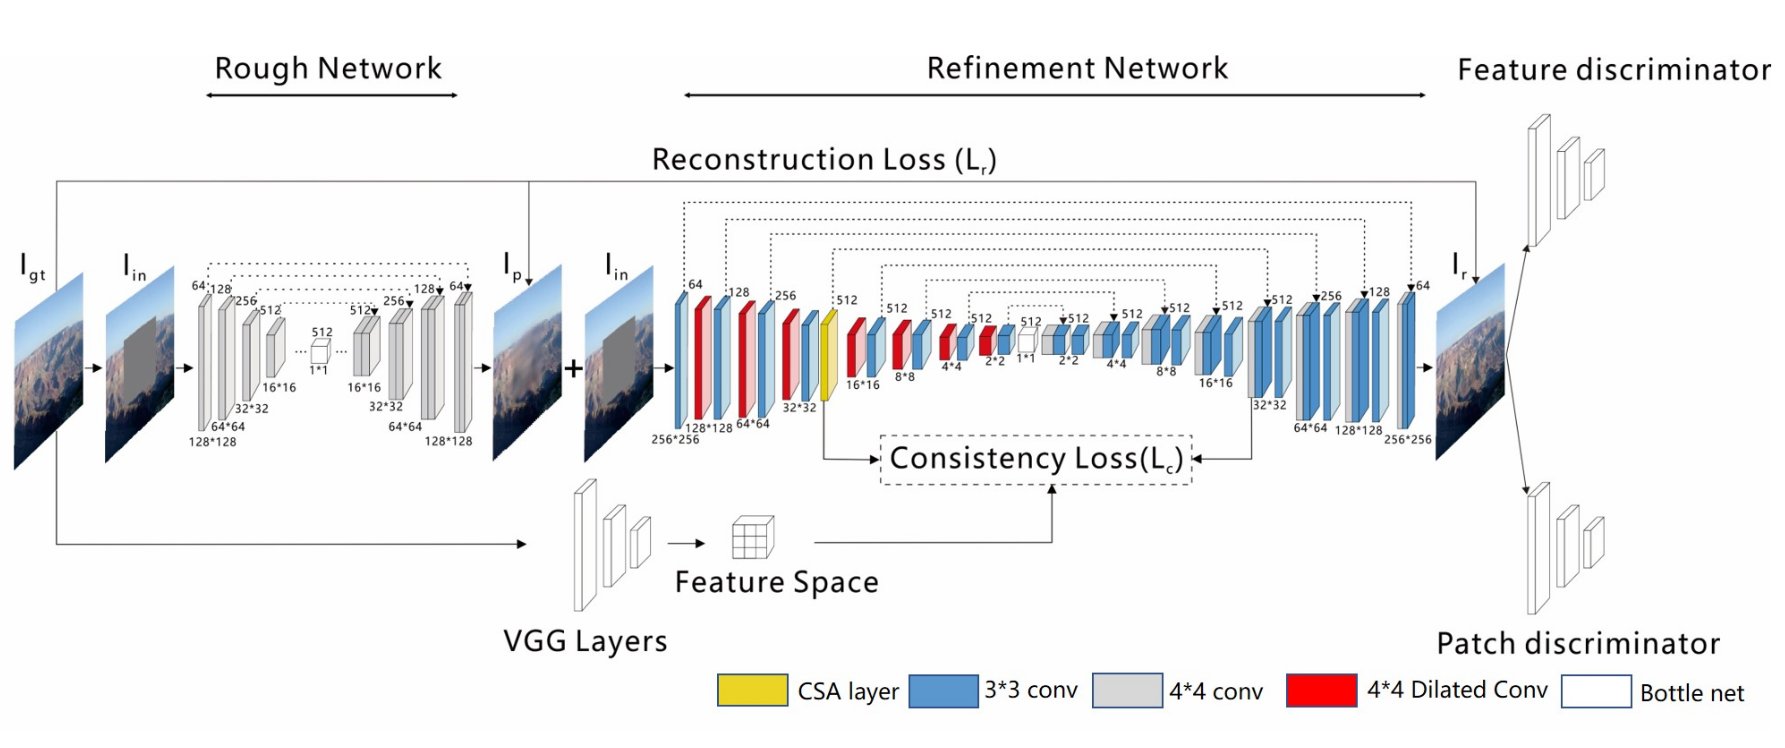
\includegraphics[width=14cm]{figures/chapter4/csa_layer.png}
    \vspace*{5mm}
    \caption{CSA layer at the resolution of \(32 \times 32\) in refinement network \cite{csa_layer}}
    \label{fig:csa_layer}
\end{figure}

In Artist-Net \cite{artistNet} proposed by Liao et al. In order to achive inpainting, two different content encoders, a style encoder used with a joint decoder. Artist-Net architecture can be seen in figure \ref{fig:artistNet}. A similar structure is also available in CNN architecture developed by Cai et al. \cite{semantic_object_removal} for the purpose of semantic object removal. There are also context encoder \cite{context_encoders} architectures used in inpainting studies. These context encoders basically CNNs trying to generate the missing parts of an image from their surroundings.

\begin{figure}[h]
    \centering
    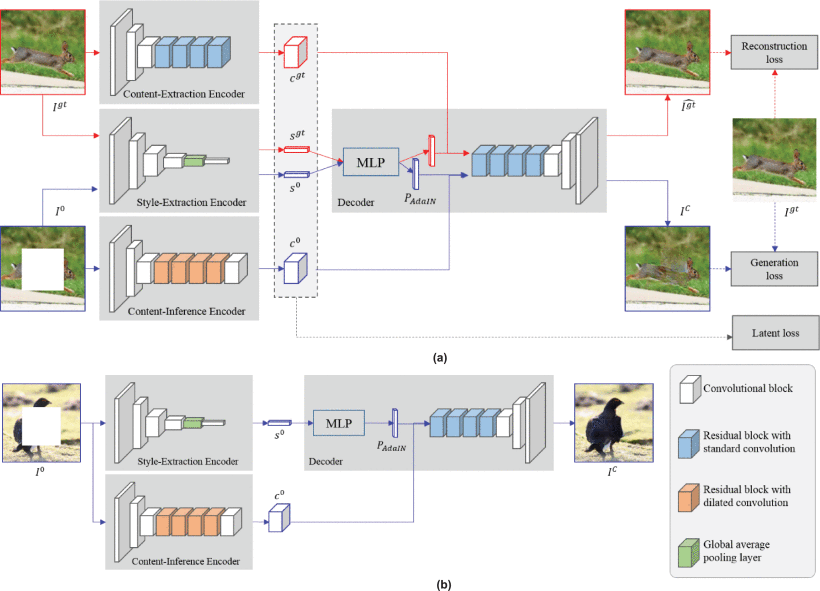
\includegraphics[width=14cm]{figures/chapter4/artist.png}
    \vspace*{4mm}
    \caption{Artist-Net Architecture \cite{artistNet}}
    \label{fig:artistNet}
\end{figure}

Zeng et al. \cite{pyramid_network} used Pyramid-context encoder network to perform inpainting. This pyramidal arthitecture called PEN-Net performs a high quality inpainting operation. The network structure can be seen in figure \ref{fig:pennet}. Nakamura et al. \cite{nakamura} aimed to remove the text from images and achieved excellent results using CNN. 

\begin{figure}[h]
    \centering
    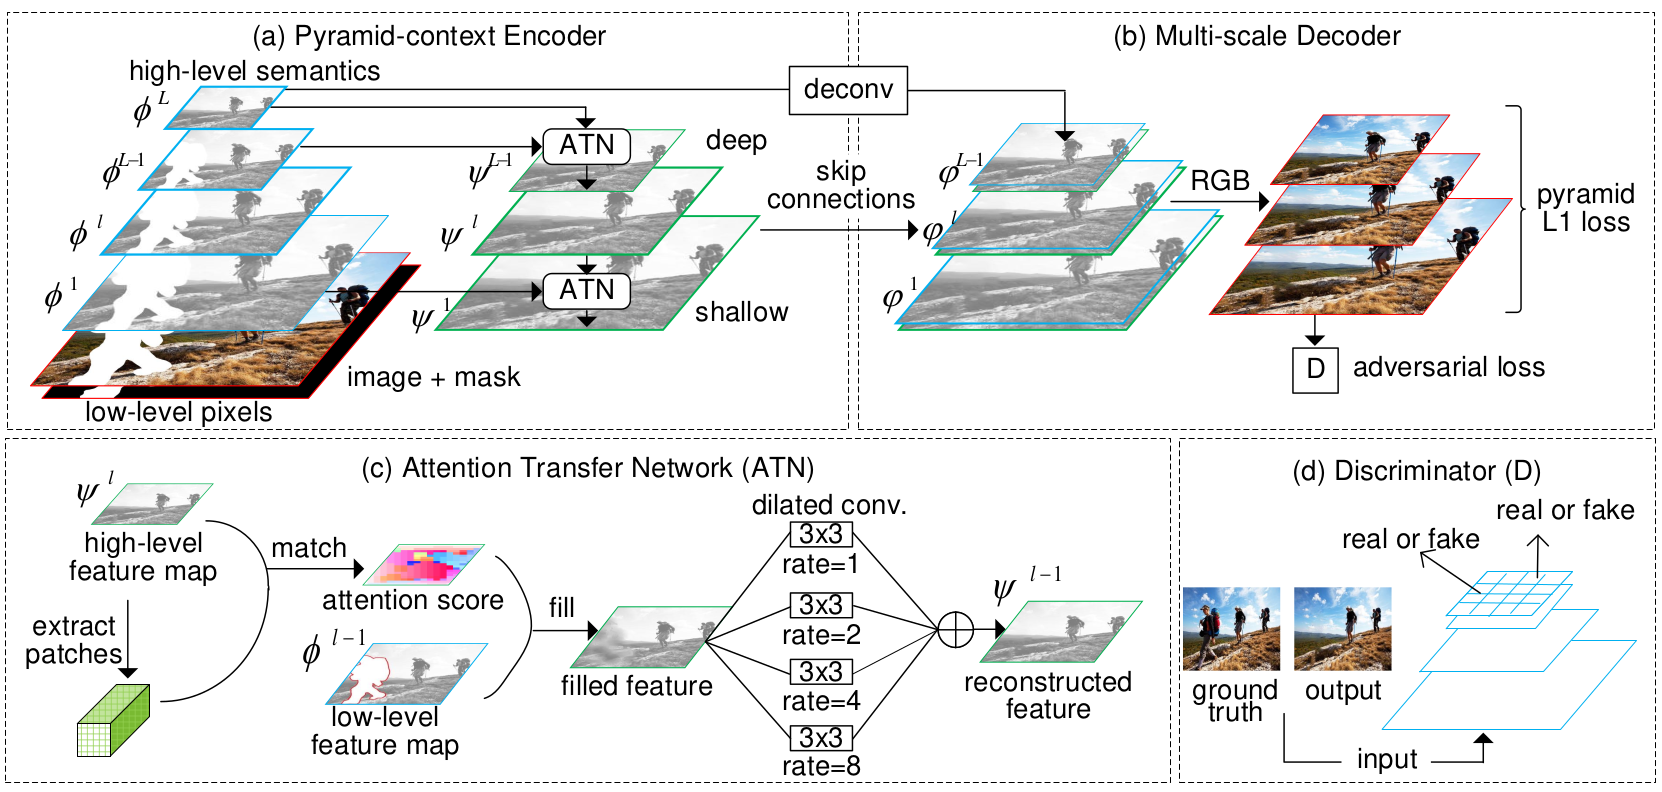
\includegraphics[width=14cm]{figures/chapter4/pyramid.png}
    \vspace*{5mm}
    \caption{The Pyramid-context Encoder Network (PEN-Net) \cite{pyramid_network}}
    \label{fig:pennet}
\end{figure}

\section{GAN-based Methods}

With different deep learning methods that have been tried over time, it has been analyzed that some methods give more successful results. It can be said that CNN and GAN based methods are better in evaluating realistic results in images. In this section, methods based on GAN idea will be explained. \newline
In the paper, Context Encoder: Feature Learning by Inpainting \cite{context_encoders}, it is shown that an encoder-decoder architecture, first create a feature space with its encoder. Then, the decoder uses that space the create realistic inpainted output image. Moreover, using different losses altogether shows significantly better and more realistic results could be constructed. Figure \ref{fig:context-encoder} illustrates the structure of Context Encoder.

\begin{figure}[h]
    \centering
    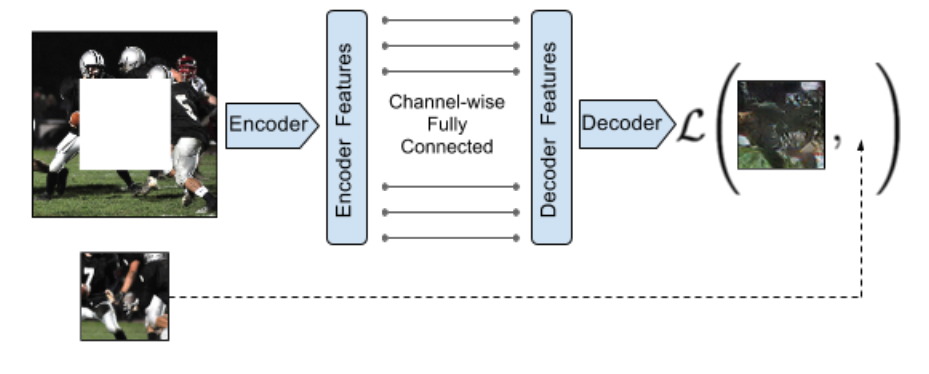
\includegraphics[scale=0.5]{figures/chapter4/context-encoder-example.png}
    \caption{Context Encoder Structure \cite{context_encoders}}
    \label{fig:context-encoder}
\end{figure}

In addition to this study, different methods have been proposed to solve different problems. To prevent blurry parts in the created pictures, using less downsampling layers are proposed by lizuka et al \cite{Iizuka2017}. Furthermore, using dilated convolution layers instead of fully connected layers are proposed by Yu and Koltun \cite{dilated_conv}. Unfortunately, these changes led to longer training times because of highly sparse filters generated by dilation element. Structure example with dilated convolution layers are presented in figure \ref{fig:dilated-model}. Gated and dilated gated convolutional layers used in a image completion study SC-FEGAN \cite{scfegan}. In this study authors built GAN-based system in order to complete masked input images with respect to the given sketches.

\begin{figure}[h]
    \centering
    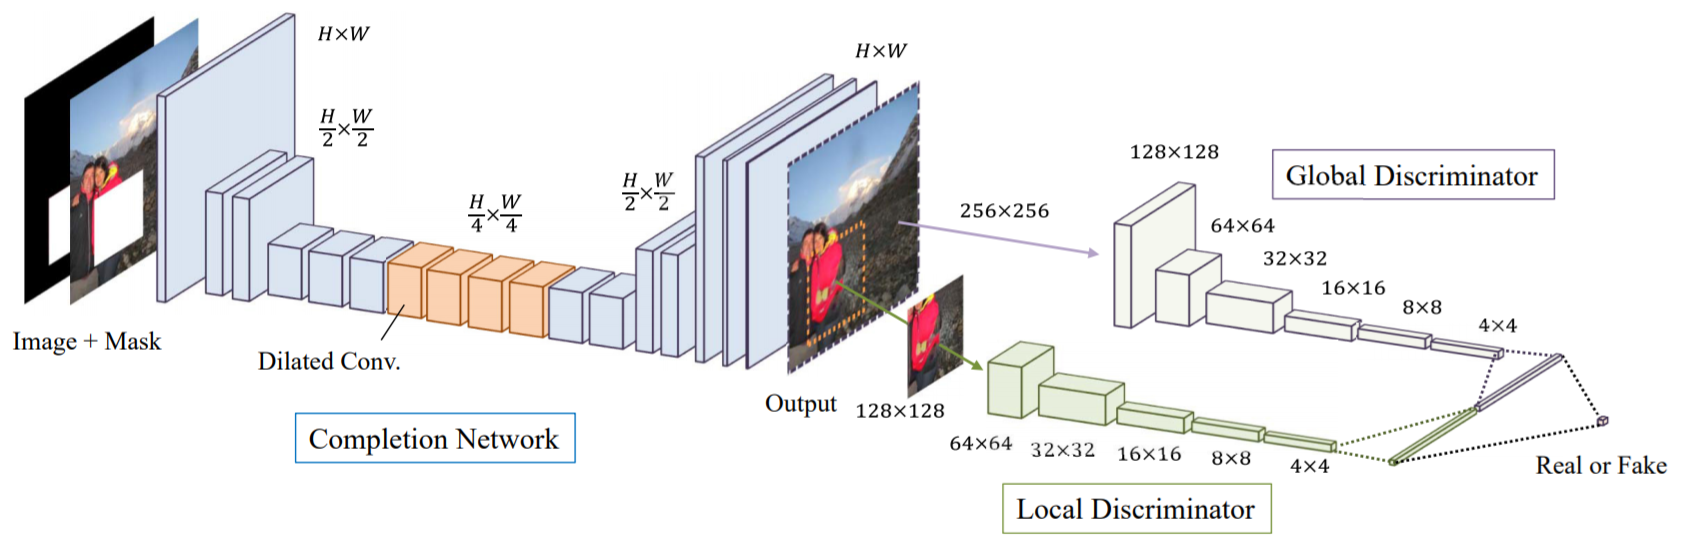
\includegraphics[scale=0.35]{figures/chapter4/Lizukaetal.PNG}
    \vspace*{5mm}
    \caption{Model with Dilated Convolution Layer \cite{dilated_conv}}
    \label{fig:dilated-model}
\end{figure}

Different methods are also used such as using a pre-trained VGG network which leads to much shorter training time, proposed by Yang et al. \cite{inpainting_neuralpatch}. Also, Liu et. Al \cite{richer_conv_edge} came up with partial convolution layers that saves convolution filters from taking too many zeros from masked regions. Partial convolution operation is shown in Figure \ref{eqn:partialconv}.

\begin{equation}
\label{eqn:partialconv}
    x^{'}= {
\begin{cases}
    W^T (X\bigodotM) \frac{sum(1)}{sum(M)}+b,& \text{if } sum(M) > 0\\
    0,              & \text{otherwise}
\end{cases}
}
\end{equation}

The novel idea that we actively use in our study and that provides the most successful results for the inpainting operation is the introduction of Generative Adversarial Networks asserted by Yeh et al \cite{semantic_inpainting_geneative}. Fundamental idea behind GAN is illustrated in Figure \ref{fig:gan-idedal} for an image related problem.

\begin{figure}[h]
    \centering
    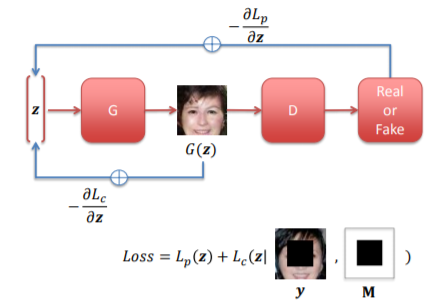
\includegraphics[scale=0.7]{figures/chapter4/GANinpainting.PNG}
    \caption{GAN Idea \cite{semantic_inpainting_geneative}}
    \label{fig:gan-idedal}
\end{figure}

Different methods that use GAN structures and add many innovations to this structure will be explained in detail in the following sections.

\newpage
\section{State-of-the-Art Methods}

\subsection{EdgeConnect}

Nazeri et al. proposed a method \cite{edgeconnect} that uses edge information to produce realistic output images over missing zones.  EdgeConnect consists of 2 different GANs placed one behind the other. The first of these GANs tries to create the missing edge information over the masked image, and the second GAN structure complements the missing image by using this created edge information and the original masked image. Fundamental idea of the structure is shown in Figure \ref{fig:edgeconnect-network}.

\begin{figure}[h]
    \centering
    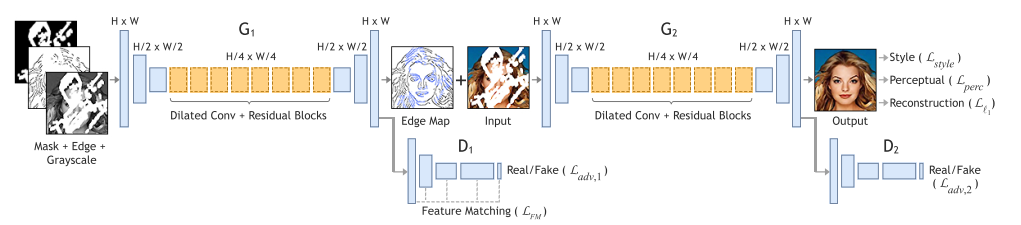
\includegraphics[scale=0.6]{figures/chapter4/EdgeConnect.PNG}
    \vspace*{5mm}
    \caption{EdgeConnect Network \cite{edgeconnect}}
    \label{fig:edgeconnect-network}
\end{figure}

With this method, Yu et al want to solve some of the basic problems that arise in the inpainting process. Using the edge information, it is desired to create visuals with sharper borders. Figure \ref{fig:edgeconnect-example} demonstrates a few examples of inpainted images with EdgeConnect.

\begin{figure}[h]
    \centering
    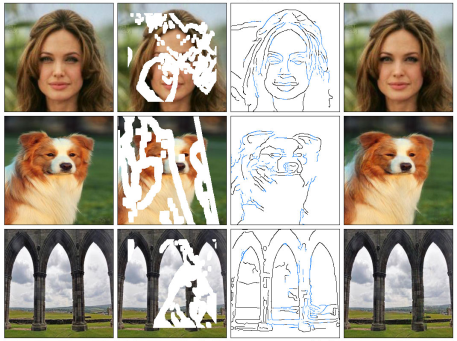
\includegraphics[scale=0.85]{figures/chapter4/ExampleEdgeConnect.PNG}
    \vspace*{5mm}
    \caption{EdgeConnect Inpainting Example \cite{edgeconnect}}
    \label{fig:edgeconnect-example}
\end{figure}

Similar features are available for both structures that create edge information and final image. Generator Network consists of 3 parts. As mentioned before, an encoder structure is used primarily for feature extraction from the image. Residual network has been added after the encoder structure. Finally, there is a decoder to produce the image from features. Convolution layers are used adjacently for the discriminator structure.
The methods, transformations and tools we use to implement these structures will be explained in detail in the following sections.\newline
The working logic of the model basically consists of 4 steps. Briefly, the image selected as input in each iteration is directed to the dataset script. In this dataset script, the process of finding an edge and separating the image from the color channels are performed. From the parts obtained in this step, the edge and gray image are given to the edge model as input. The output is reverse masked and summed with the original parts. In this way, we only get the part produced about the masked region of the output picture. Then, with the edge information obtained from this section, the RGB image is given to the inpainted model and again reversely masked. \newline
Our goal was to implement the same model into our framework. To achieve this purpose, we got inspired by the example models that are publicly shared on internet. This was one of the main challenges on our project.  


\subsubsection{Edge Generator}

Edge generation is the fundamental idea behind EdgeConnect. In this section, generating edge will be explained.
Input image that is given to the system will be denoted as \(I_{gt}\), which stands for ground truth image. Also, edge information of input image and gray scale version of input image are denoted as \(C_{gt}\), \(I_{gray}\) respectively. Hence, while masked version of edge information and gray scale input images are represented as \(I^m_{gray}=I_{gray} \bigodot (1-M)\)  and \(C^m_{gt}=C_{gt}\bigodot(1-M)\), edge generation can be expressed as equation \ref{eqn:edge1}. In these operations, \(\bigodot\) represents Hadamard product.

\begin{equation}
\label{eqn:edge1}
    C_{pred} = G_{1}(I^{m}_{gray}, C^{m}_{gt}, M)
\end{equation}

\(C_{gt}\) and \(C_{pred}\) is given to discriminator network along with \(I_{gray}\), which tries to predict if the given edge map is real. In a greater scale whole network is trained using an objective function which is given in equation \ref{eqn:edge2} with adversarial loss and feature loss.

\begin{equation}
\label{eqn:edge2}
    min_{G_{1}}max_{G_{2}}\mathcal{L}_{G_{1}} = min_{G_{1}}(\lambda_{adv,1}max_{D_{1}}(\mathcal{L}_{adv,1})+\lambda_{FM} \mathcal{L}_{FM})
\end{equation}

In above equation, \(\lambda_{adv,1}\) and \(\lambda_{FM}\) are called regularization parameters and they are adversarial loss and feature matching loss respectively. Adversarial loss is given equation \ref{eqn:edge3}.

\begin{equation}
\label{eqn:edge3}
    \mathcal{L}_{adv,1} = \mathbb{E}_{(C_{gt},I_{gt})}[logD_{1}(C_{gt},I_{gray})]+\mathbb{E}_{I_{gray}}log[1-D_{1} (C_{pred}, I_{gray})]
\end{equation}

Feature-matching loss, pushes network to generate images more similar to real images from dataset which helps network to be more stable. Feature matching loss is given in equation \ref{eqn:edge4} below.

\begin{equation}
\label{eqn:edge4}
    \mathcal{L}_{FM} = \mathbb{E} [ \sum\limits^L_{i=1}{\frac{1}{N_i}|| D_1^(i) (C_{gt}-D_1^{i} (C_{pred})) ||_1} ]
\end{equation}

In given equation, \(N_i\) represents the number of elements in the activate layer numbered with i. \(D_1^{(i)} \) is discriminator’s activation in layer i and L is the discriminator’s last layer.

\subsubsection{Image Completion Network}

Inpainting network uses masked image which is expressed as  \(I^m_{gt}=I_{gt} \bigodot(1-M)\) to produce inpainted images over masked areas. Inpainting network also uses composite edge map which is defined as \(C_{comp}=C_{gt}  \bigodot (1-M)+C_{pred}  \bigodot M.\) Using these inputs, network produces an output with filled missing regions shown in equation \ref{eqn:edge5}.

\begin{equation}
\label{eqn:edge5}
    I_{pred} = G_2 (I^m_{gt}, C_{comp})
\end{equation}

Overall, image completion network is trained with joint losses which are \(\iota_1\) loss, adversarial loss, perceptual loss and style loss. Similar in edge generator adversarial loss is shown in equation \ref{eqn:edge6}. 

\begin{equation}
\label{eqn:edge6}
    \mathcal{L}_{adv,2} = \mathbb{E}_{(I_{gt},C_{comp})}[logD_{2}(I_{gt},C_{comp})]+\mathbb{E}_{C_{comp}}log[1-D_{2} (I_{pred}, C_{comp})]
\end{equation}

Other two losses that is used in image completion network is proposed in \cite{style} and \cite{perceptual} known as \(L_{perc}\)\space and \space \(L_{style}\).  Perceptual loss, penalizes the generated images if they are not similar perceptually to activation maps of a network that is trained before. Perceptual loss is shown in equation \ref{eqn:edge7}, where \(\phi_i\) is the activation map of pre-trained network on i’th layer.

\begin{equation}
\label{eqn:edge7}
    \mathcal{L}_{perc} = \mathbb{E}[ \sum\limits_{i=1}\frac{1}{N_i} || \phi_i(I_{gt}-\phi_i (I_{pred}) ) ||_1 ]
\end{equation}

Activation maps that are used in perceptual loss are also used in style loss which is expressed in equation \ref{eqn:edge8}.

\begin{equation}
\label{eqn:edge8}
    \mathcal{L}_{style} = \mathbb{E}_j [ || G_j^{\phi} (I^m_{pred})- G_j^{\phi} (I^m_{gt}) ||_1 ]
\end{equation}

\(G_j^\phi\) is Gram matrix that is obtained from previously shown activation matrix. Finally, overall loss function of the system is given in equation \ref{eqn:edge9}.

\begin{equation}
\label{eqn:edge9}
    \mathcal{L}_{G_2}=\lambda_{l_1}\mathcal{L}_{l_1} + \lambda_{adv,2}\mathcal{L}_{adv,2} + \lambda_{perc}\mathcal{L}_{perc} + \lambda_{s}\mathcal{L}_{style}
\end{equation}

\subsection{Generative Image Inpainting with Contextual Model}

One of the main problems in inpainting methods is that they create blurry and distorted parts in the missing regions. To prevent this, Yu et al. came up with Generative Image inpainting with Contextual Attention \cite{generative_contextual}.
Generative image inpainting with contextual attention consists of 2 main stages which are called Coarse Network and Refinement Network. Model structure is illustrated in figure \ref{fig:contextual-structure}.

\begin{figure}[h]
    \centering
    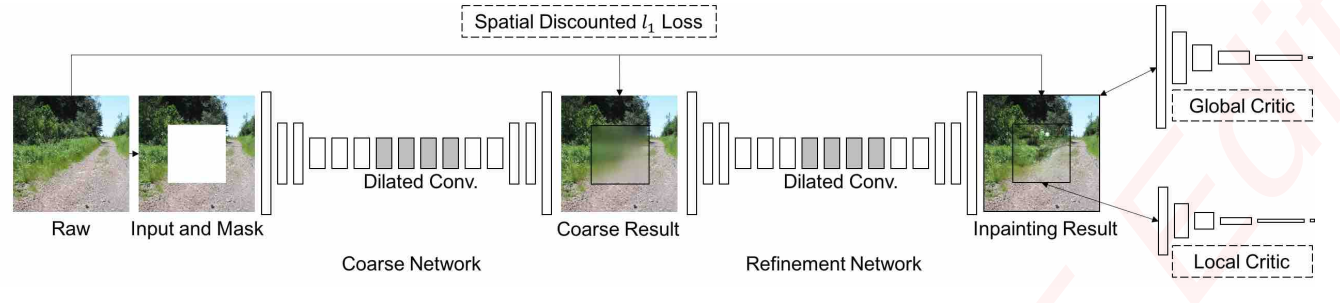
\includegraphics[scale=0.4]{figures/chapter4/GenerativeOverview.PNG}
    \vspace*{3mm}
    \caption{Contextual Attention Model Structure \cite{generative_contextual}}
    \label{fig:contextual-structure}
\end{figure}

Coarse Network uses a method similar to the encoder and decoder structure like many methods previously described. In this part, an inpainted image is created over the missing part by using the GAN structure. \newline
The main idea of this study lies in Refinement network. The image created in this section progresses on 2 different paths, then the outputs of these 2 different paths are combined to achieve the desired improved result. Refinement network is shown in more detail in figure \ref{fig:refinement-network}.

\begin{figure}[h]
    \centering
    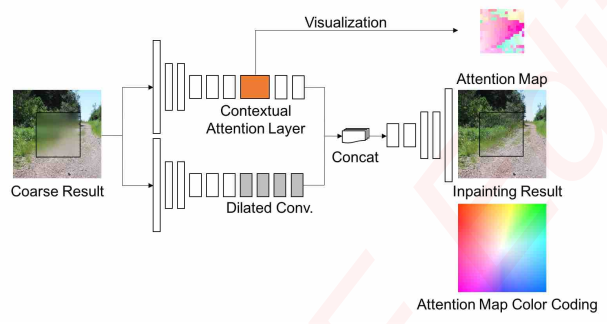
\includegraphics[scale=0.85]{figures/chapter4/GenerativeAttention.PNG}
    \caption{Refinement Network \cite{generative_contextual}}
    \label{fig:refinement-network}
\end{figure}

In the first of these 2 paths, there is a structure consisting of dilated convolution and normal convolution layers. In the other and more important structure, there is a layer called Contextual Attention Layer that performs attention perception through the color map on the picture. In this layer, the picture is divided into patches and compared and evaluated. Algorithm in attention scoring is explained in Figure \ref{fig:attention-scoring}.

\begin{figure}[h]
    \centering
    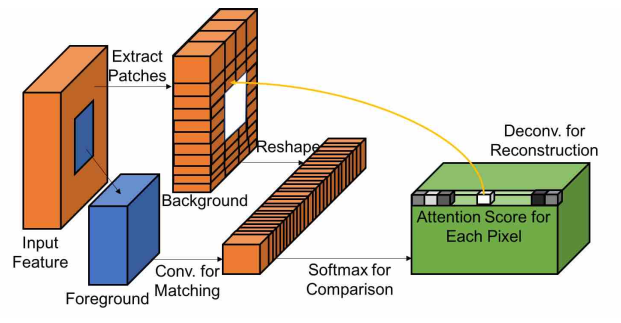
\includegraphics[scale=0.85]{figures/chapter4/GenerativeScoring.PNG}
    \caption{Refinement Network \cite{generative_contextual}}
    \label{fig:attention-scoring}
\end{figure}

The Generative Contextual Attention Model has common similarities with the Edge connect model in terms of training. But there are critical differences due to the model type as expected. 

\subsubsection{Contextual Attention}

Contextual attention layer can fill the masked areas by using the feature information obtained from the unchanged parts of the image. For this, firstly, it divides the unmasked region expressed as background into patches and organizes it as a convolutional filter. Then it is put into the cosine similarity operation shown in equation [] with patches in the masked region expressed as foreground.

\begin{equation}
\label{eqn:context}
    s_{x,y,x^{'},y^{'}} = <\frac{f_{x,y}}{||f_{x,y}||}, \frac{b_{x^',y^'}}{||b_{x^{'},y^{'}}||}>
    % NEDEN HATA VERIYOR
\end{equation}

Where \(s_{x,y,x^{'},y^{'}}\) is patch similarity between background and foreground. Following this step, softmax function is used to obtain a similarity score with constant value \(\lambda\), as \(s^{*}_{x,y,x^{'},y^{'}} = softmax_{x^{'},y^{'} } ( \lambda_{s_{x,y,x^{'},y^{'} } } )\). In final step, used background patches are reused as deconvolutional filters to reconstruct foregrounds. For better results, attention coherency could be increased by calculating a new attention score by summing scores in a shifted direction in desired axis.

\subsection{Image Inpainting via Generative Multi-column CNN}

In the article \cite{inpainting_via_multi_cnn}, the inpainting process is presented with a multi column CNN structure. This network acquires different image features in parallel. A new reconstructon loss function has been developed to better characterize global objects. Also, a loss function called ID-MRF loss has been developed to increase the local details and improve the texture quality. With these loss functions and a adversarial loss, the model trained on the image dataset can fill the masked pixels in an image with local and global information. Trained model of this architecture shows realistic results without even the need for post-processing, which is often seen on similar works.

This inpainting system has a structure that can be trained from begining to end. It first receives an image and a binary mask as input. The pixels to be masked are denoted by 1 and known pixels by 0. Then the image masked by the  operation and inserted into the network. The result of the network is a completed image. Network structure is as shown in the figure \ref{fig:gmcnn}.

\begin{figure}[h]
    \centering
    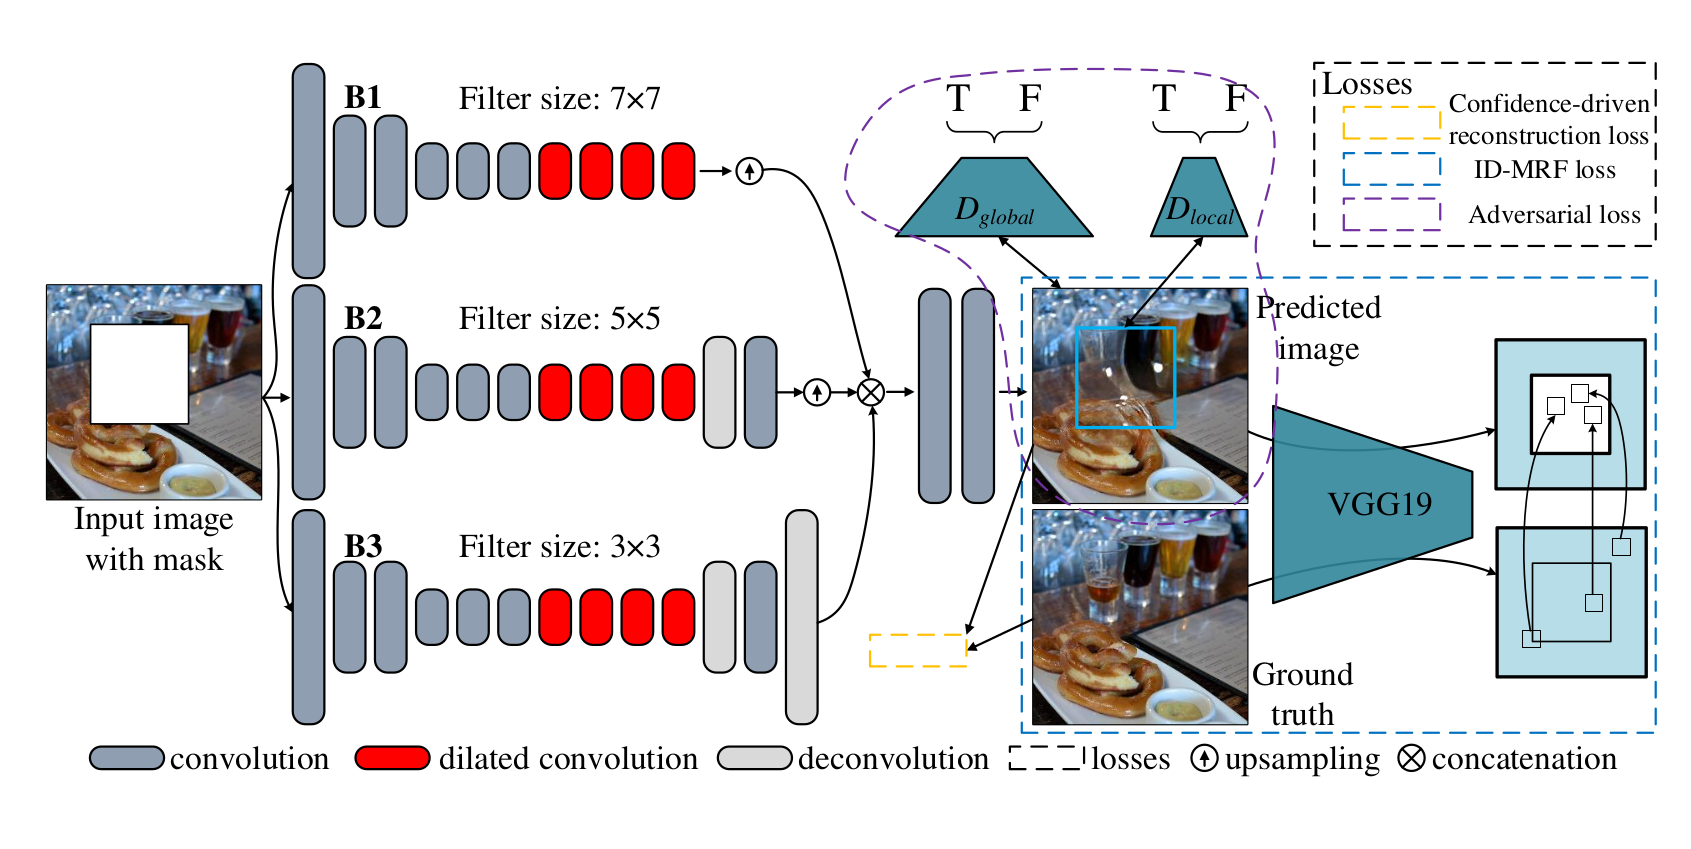
\includegraphics[width=14cm]{figures/chapter4/gmcnn.png}
    \caption{Network structure of the GMCNN \cite{inpainting_via_multi_cnn}}
    \label{fig:gmcnn}
\end{figure}

The network structure shown in figure \ref{fig:gmcnn} consists of three sub-networks. The first one is the generator network that creates the output inpainted image and is the main network which will used after the training phase. The other two sub-networks are networks that are only needed during the training phase respectively, local and global discriminator networks which used to calculate the adversarial loss and a pre-trained VGG network \cite{very_deep_conv} in order to calculate the designed ID-MRF loss. Generator network consists of n parallel encoder-decoder branches (in figure \ref{fig:gmcnn}, n = 3). These structures consist of convolution layers that apply filters of different kernel sizes to the input tensor. These convolution layers obtain features at different frequency levels according to the kernel size. Next, these branches which have different levels of information about input image upsampled bilinearly to the original image size. Then these same size branches combined together and forms a feature map. Continued with two more convolution layers, this feature map is transformed into the image. This image is the generated output image of the network and it is used to calculate the network loss when compared to the ground truth image. Even though these branches seem to be independent from each other, they are actually affected by the backpropagation phase in the training process. This framework is different from the commonly used encoder-decoder structures. In an encoder-decoder network, every layer inherits its information from its previous layer. However, in this architecture, different structures complement each other instead of just inheriting. With these different representation levels, the inpainting process is carried out.

To calculate loss during model training, a mixture of three loss functions used. ID-MRF loss, reconstruction loss, and adversarial loss.

ID-MRF stands for implicit diversified Markov random fields. This loss function is used to train with a path similarity based approach within a VGG structure fed with generated results. This method, which is used only during the training phase, is a metric used to measure the similarity between the randomly selected patches between generated pixel areas and the ground truth area pixel areas. A simple similarity measure like cosine similarity can be used to compute this process. This metric measures the similarity between the generated content and the random selected nearest-neighbor patches. But using cosine similarity measurement has some limitations. As seen in the figure \ref{fig:cosine_similarity}.a, the results often become like blurry textures and for large masking areas this can become a serious problem.

\begin{figure}[h]
    \centering
    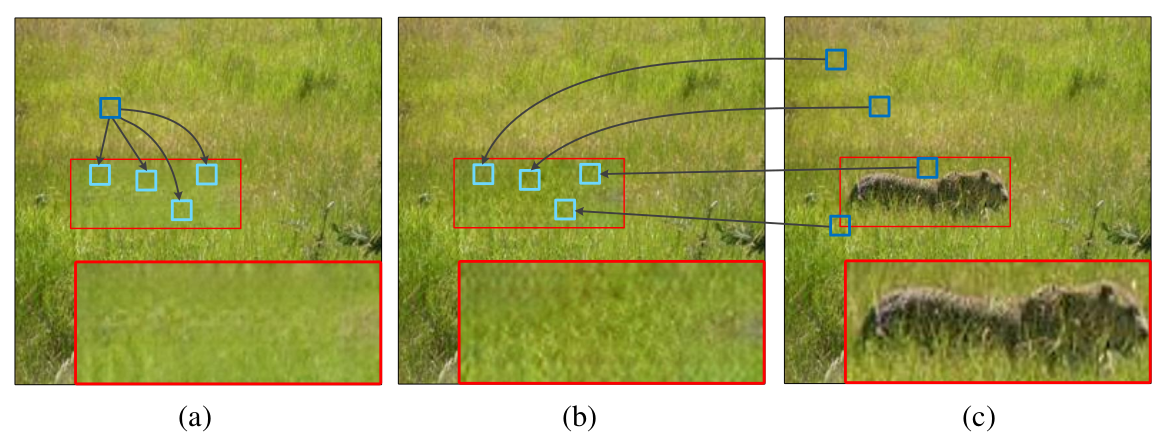
\includegraphics[width=13cm]{figures/chapter4/cosine_similarity.png}
    \caption{Cosine similarity vs. Relative similarity \cite{inpainting_via_multi_cnn}}
    \label{fig:cosine_similarity}
\end{figure}

In this article, in order to eliminate this problem, a relative similarity measurement has been developed and used instead of a direct similarity such as cosine similarity. As seen in figures \ref{fig:cosine_similarity}.b and \ref{fig:cosine_similarity}.c, the ground truth image pathches compared with the generated image patches. This relative similarity equation can be seen in equation \ref{eq:relative_similarity}.

\begin{equation}
    RS(v, s) = exp((\frac{\mu (v, s)}{\max_{r\in \rho_{v} (Y^{L}))} \mu(v,r) + \epsilon }) / h)
    \label{eq:relative_similarity}
\end{equation}

\(\mu (v, s)\) in the equation represents cosine similarity between patch \(v\) from generated area and patch \(s\) from ground truth area, the  and  values are constants, and  represents the features on the \(L^{th}\) layer of the pre-trained VGG network. To be more precise, let generated content denoted as and is the corresponding ground truth, for any layer L, ID-RMF loss can be calculated as equation in the equation \ref{eq:idrmf_loss}.

\begin{equation}
    \mathfrak{L}_{M}(L) = - log(\frac{1}{z} \sum_{s \in Y^{L}} \max_{v \in \widehat{Y}_{g}^{L}} \overline{RS} (v, s))
    \label{eq:idrmf_loss}
\end{equation}

The \(\overline{RS}\) is the normalized relative similarity as in the equation \ref{eq:normalized_rs} and \(Z\) is normalization factor. \(r\) and \(s\) represents the patches from generated image and ground truth image respectively.

\begin{equation}
    \overline{RS}(v,s) = RS(v,s) / \sum_{r \in \rho_{v}(Y^{L})} RS(v,r)
    \label{eq:normalized_rs}
\end{equation}

If all \(r\) patches in the \(\widehat{Y}_{g}^{L}\) are close to only one spesific patch and far from other patches in ground truth, relative similarity becomes small and leads to a big loss value \(\mathfrak{L}_{M}(L)\). On the other hand if every \(r\) patch from generated image has a similar corresponding \(s\) patch in ground truth image, relative similarity becomes big and leads to a small loss value. One of the biggest contributions of this measure is to increase the similarity between the \(Y^{L}\) and \(\widehat{Y}_{g}^{L}\) features. While minimizing the loss, generated feature distrubution and ground truth feature distrubution approach each other. As a result, in the inpainting regions blurry texture problem is overcome and variation is achieved.

\begin{equation}
    \mathfrak{L}_{mrf} = \mathfrak{L}_{M}(conv4 \_ 2) + \sum_{t = 3}^{4} \mathfrak{L}_{M}(conv \mathbf{t} \_ 2)
    \label{eq:Lmrf}
\end{equation}

With this loss active, during the training phase, a realistic texture was obtained both locally and globally. The features layers mentioned and shown in the equation \ref{eq:Lmrf} are taken from the VGG19 pre-trained model \cite{very_deep_conv}.

A pixel-wise working reconstruction loss has been developed as a spacial variant reconstruction loss. In this designed confidence-driven reconstruction loss, known pixel values assigned with the value of 1 and others missing pixels confidence values gradually decays with respect to the distance from the mask border. Thus the pixels on the boundary make the most impact on the loss. As a result, a smooth transition between the masked area and the rest of the image is achieved. Increasing distance away from the boundary is obtained by convolving the mask with a gaussian filter and formulized like equation \ref{eq:gaussian_filter}.

\begin{equation}
    M_{\omega}^{i} = (g \ast \overline{M}^{i}) \odot M
    \label{eq:gaussian_filter}
\end{equation}

\(g\) represents a \(64 \times 64\) gaussian filter with standart deviation of 40 and \(\odot\) is the Hadamard product operator. Hadamard product means element-wise multiplication of the matrices. Loss weight mask \(M_{\omega}\) is obtained by repeating the equation \ref{eq:gaussian_filter} several times. Lastly the reconstruction loss calculated with the formula in \ref{eq:reconstruction_loss}.

\begin{equation}
    \mathfrak{L}_{c} = \left \| (Y - G([X, M]; \theta )) \odot M_{\omega} \right \|_{1}
    \label{eq:reconstruction_loss}
\end{equation}

In equation \ref{eq:reconstruction_loss}, \(G([X, M]; \theta )\) represents the generated output. With the help of this loss, the results are softened from the mask boundaries towards the center.

Adversarial loss is used frequently in many tasks such as inpainting missing pixels. In this architecture, improved Wasserstein GAN \cite{improved_train_wgan} is used as a generator and one local and one global structure are used together as a discriminator. Reason for using two discriminators is to overcome the problem when generated areas are realistic and low loss but ill-matched with the rest of the image. The adversarial loss function is defined as in equation \ref{eq:adversarial_loss}, where \(\widehat{X} = tG([X, M]; \theta) + (1 - t) Y\) and \(t \in [0, 1]\).

\begin{equation}
    \mathfrak{L}_{adv} = - E_{X \sim \mathbb{P}_{x}}[D(G(X;\theta))] + \lambda_{gp} E_{\widehat{X} \sim \mathbb{P}_{\widehat{x}}}[(\left \| \nabla_{\widehat{X}} D(\widehat{X}) \odot M_{\omega} \right \|)_{2} - 1)^{2}]
    \label{eq:adversarial_loss}
\end{equation}

Finally, the three loss functions mentioned above are combined together with different weights denoted as \(\lambda_{mrf}\) and \(\lambda_{adv}\) in equation \ref{eq:total_loss}. Regularization of the model achieved in training process.

\begin{equation}
    \mathfrak{L} = \mathfrak{L}_{c} + \lambda_{mrf} \mathfrak{L}_{mrf} + \lambda_{adv} \mathfrak{L}_{adv}
    \label{eq:total_loss}
\end{equation}

As a comparison with GMCNN, two other CNN-based inpainting architectures selected under same conditions with the same losses and same hyperparameters. A single encoder-decoder network and the previously mentioned contextual attention coarse network \cite{generative_contextual} tested alongside with the GMCNN. Results are shown in figure \ref{fig:gmcnn_paris_comparison}. In \ref{fig:gmcnn_paris_comparison}.b, output of a single encoder-decoder network is shown. In \ref{fig:gmcnn_paris_comparison}.c, output of the contextual attention
coarse network is shown. Lastly, in figures \ref{fig:gmcnn_paris_comparison}.d and \ref{fig:gmcnn_paris_comparison}.e output of the GMCNN can be seen. Yhe former is the network with the fixed receptive fields and the latter is with varied receptive fields.

\begin{figure}[h]
    \centering
    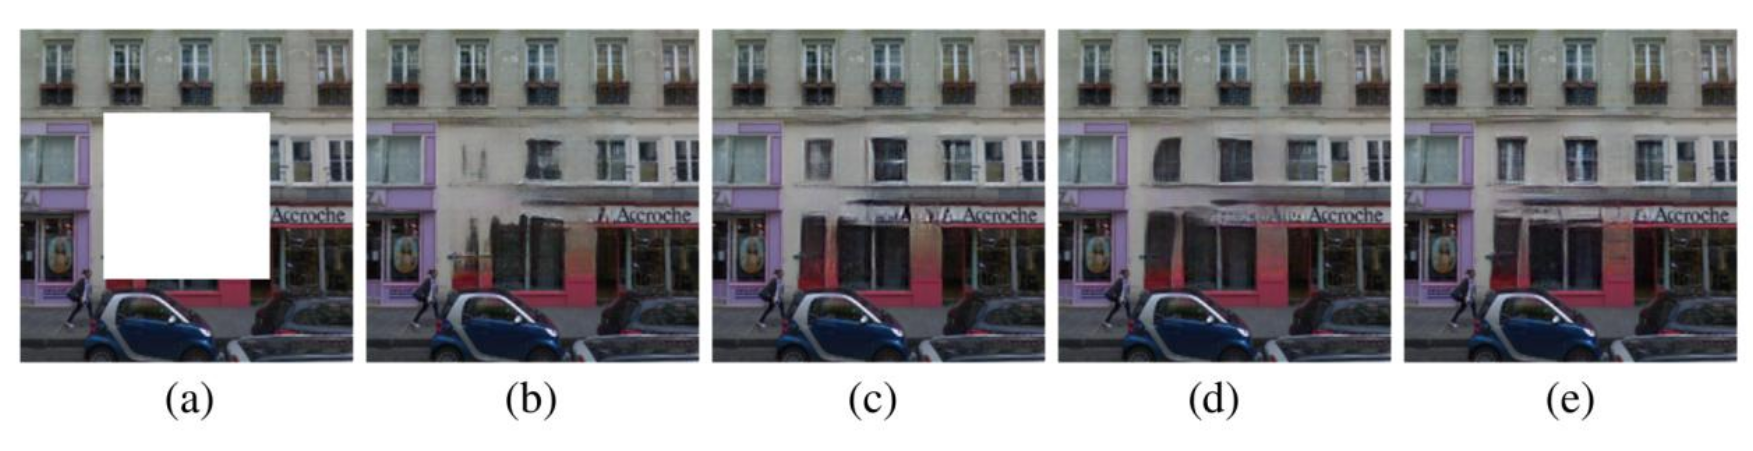
\includegraphics[width=14cm]{figures/chapter4/gmcnn_paris_comparison.png}
    \caption{Comparison between GMCNN and CNN-based methods \cite{inpainting_via_multi_cnn}}
    \label{fig:gmcnn_paris_comparison}
\end{figure}

Also our results with the GMCNN using a pretrained network, achieved great looking outputs with two different datasets. Places \cite{dataset_places} dataset and CelebA \cite{celebA} dataset outputs can be seen in the figures \ref{fig:gmcnn_places2} and \ref{fig:gmcnn_celebA} respectively.

\begin{figure}[h]
    \centering
    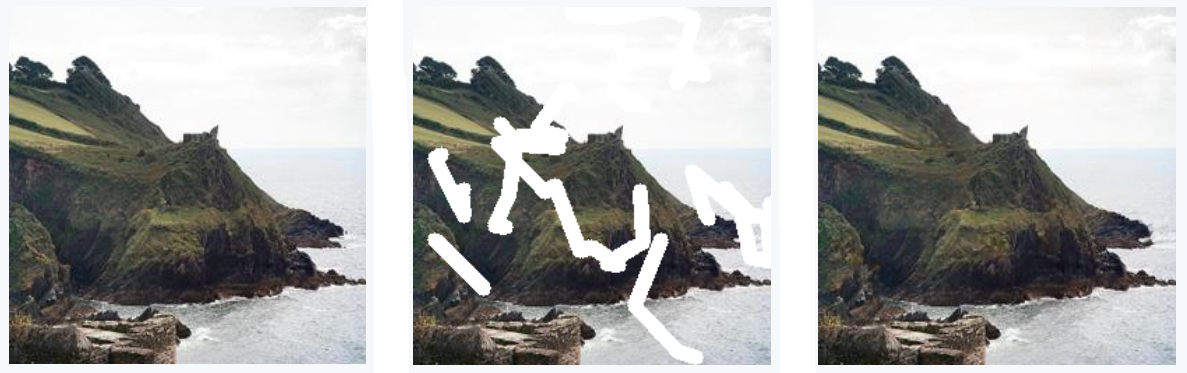
\includegraphics[width=14cm]{figures/chapter4/gmcnnout2.png}
    \vspace*{3mm}
    \caption{Result of the model trained on Places2 dataset}
    \label{fig:gmcnn_places2}
\end{figure}

As a limitation, like most of the generative neural networks this network also struggle with large datasets with diverse classes such as ImageNet. It is a harsh challange to inpaint different objects and places with one pre-trained model.

\begin{figure}[h]
    \centering
    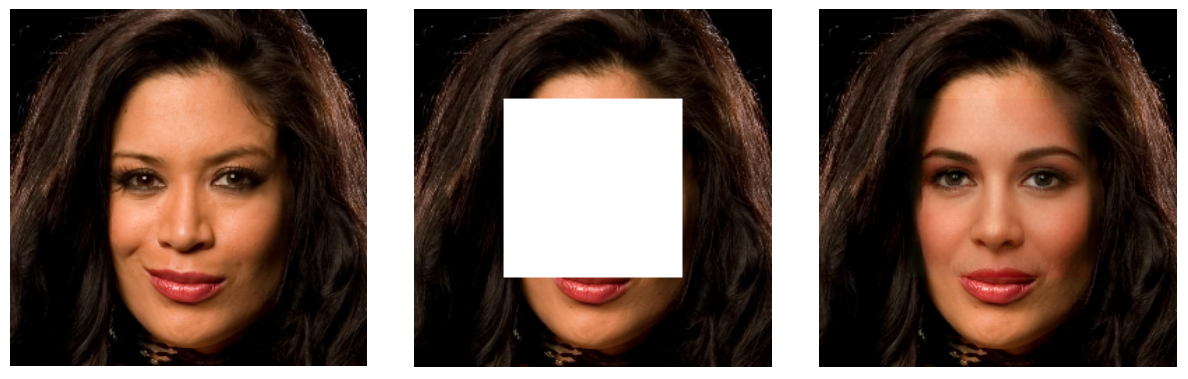
\includegraphics[width=14cm]{figures/chapter4/gmcnnout1.png}
    \vspace*{3mm}
    \caption{Result of the model trained on CelebAHQ dataset}
    \label{fig:gmcnn_celebA}
\end{figure}

\subsection{Deep Image Prior}

Deep convolutional networks have become very popular for image generation and restoration problems. In general, the reason behind the good results of such networks is the ability to obtain realistic image priors from datasets containing large number of images. To explain briefly what image prior is, it is a general definiton for the information on an image that can be used for any kind of image processing tasks to enhance results, to choose the processing parameters, and resolve indeterminacies. For instance, some information about an image may known such as color distrubution, and this information or its approximation can be used as a prior to a spesific task. Image priors can be represented with math form and merged into processing steps such as filtering, deconvolution and segmentation which helps to reduce the feasible solutions.

In the article \cite{deep_image_prior}, the authors show that a generator network structure can get enough low-level image statistics without a long training phase on any dataset. To prove this hypothesis, designed deep image prior method with a randomly-initialized convolutional neural network was used as a prior and highly competitive results were obtained in various inverse computer vision problems such as denoising, super-resolution, and image inpainting. What makes this method important except that it can be used in a wide range of cumputer vision research areas, it can also forms a new branch between learning-based networks and learning-free networks with fixed explicit priors like self-similarity etc. To be declared in a single sentence, in deep image prior, authors tries to bridge the gap between two popular methods by constructing a new explicit prior using convolution neural network.

To perform the task of image restoration like inpainting, learned-prior and explicit-prior are the two common methods utilized by researchers. To explain with an example, learned-prior is a straight forward approach to train a deep convolution network to learn about the world through the dataset. On the other hand, explicit-prior or hand-crafted prior method, is embedding constrains and distinctly teaching what types of images are natural. However in real word it is extremely difficult to express constraints mathematically. As a result, most of the explicit-prior methods works poorly compared to a state-of-the-art pre-trained neural network, yet deep image prior method offers surprisingly good results which can compete with learned-prior methods.

Deep convolutional networks are architectures that on of the best for solving inverse image problems. Architectures like generative adversarial networks and variational auto-encoders achieve state-of-the-art solutions on this tasks. However, it is not entirely correct to assume that the reason for the amazing results of these models trained on large datasets is that they can capture realistic image priors while learning over the data. Because only a good learning curve on a selected datasets does not prove that a network performs good on an image from a different dataset. A good network requires generalization which means that the structure of the network should resonate with the structure of the given input data \cite{deep_image_prior}. For example, an image classification network which successfully generalized for real data can overfit when a random labels are presented \cite{understanding_deeplearning}.

To put it more clearly, in this article the authors shows that learning process is not a requirement and it is possible to obtain quite good image priors with a convolutional generative structure that does not need training. In order to prove this claim, an untrained, randomly-initialized convolutional generator neural network is fitted on a given corrupted image. Generator network initialized with a random distrubution conditioned to the input corrupted image. The reconstruction task is expressed as a conditional image generation problem. Randomly initialized network weights optimized without needing any other data than input image and network itself. Only prior information is in the structure of the network itself. \cite{deep_image_prior} as authors states.

\begin{equation}
    x = f_{\theta}(z), \hspace{5mm} x \in R^{3\times H \times W}, \hspace{5mm} z \in R^{C'\times H' \times W'}
    \label{eq:prior_mapping}
\end{equation}

In equation \ref{eq:prior_mapping}, \(x\) is corrupted input image, \(z\) is a code tensor and  represents the network parameters which randomly initialized in the beginning and will map code tensor \(z\) to the image \(x\) while resolving inverse problem through iterations. The network is switching between filtering operations such as non-linear activation, convolution, and upsampling. For most of the experiments, a hourglass type U-Net architecture with two million parameters used \cite{deep_image_prior}, \cite{hourglass}.

In image restoration problems the goal is to recover original image \(x\), when having a corrupted image \(x_{0}\). To solve such tasks, problem is often formulated as an optimization like in equation \ref{eq:prior_min}.

\begin{equation}
    x^{\ast} = \min_{x} E(x;x_{0}) + R(x)
    \label{eq:prior_min}
\end{equation}

In equation \ref{eq:prior_min}, \(E(x;x_{0})\) is a data term dependent to the task and \(R(x)\) is an image prior. For a wide range of problems, such as super-resolution, denoising, and inpainting, the data term is typically simple to design, while designing the image prior is a challenging. For inpainting problems, the corresponding data term is defined as in the equation \ref{eq:prior_dataterm}.

\begin{equation}
    E(x;x_{0}) = \left \| (x - x_{0}) \odot m \right \|^{2} , \hspace{5mm} m \in \{0, 1\}^{H \times W}
    \label{eq:prior_dataterm}
\end{equation}

The symbol \(\odot\) is the Hadamard product operator which was explained in former sections and \(m\) is the binary mask applied onto ground truth image \(x\). The goal is to reconstruct the ground truth image \(x\) from the given image \(x_{0}\)  with missing pixel values.

As mentioned, choosing a regularizer \(R(x)\) that can catch general priors in image \(x\) is a difficult and very extensive research subject within itself. To give an example, if total variation (TV) \cite{deep_inverting} is selected as a regularizer, the results are often have uniform regions. In this study, as seen in the equation \ref{eq:prior_theta}, implicit prior which gathered from neural network was used as a regularizer.

\begin{equation}
    \theta_{\ast} = \argmin_{\theta}E(f_{\theta}(z);x_{0}) , \hspace{5mm} x^{\ast} = f_{\theta^{\ast}}(z)
    \label{eq:prior_theta}
\end{equation}

\(\theta^{\ast}\) is the minimizer achieved with the help of the gradient descent optimizer from random parameter values. Result of the inpainting process denoted as \(x^{\ast}\) is given in equation \ref{eq:prior_theta}. It is also possible to apply minimazation on the code tensor \(z\). However here \(z\) is a fixed three dimensional tensor containing 32 feature maps of uniform noise with the same spatial size as \(x\).

\begin{figure}[h]
    \centering
    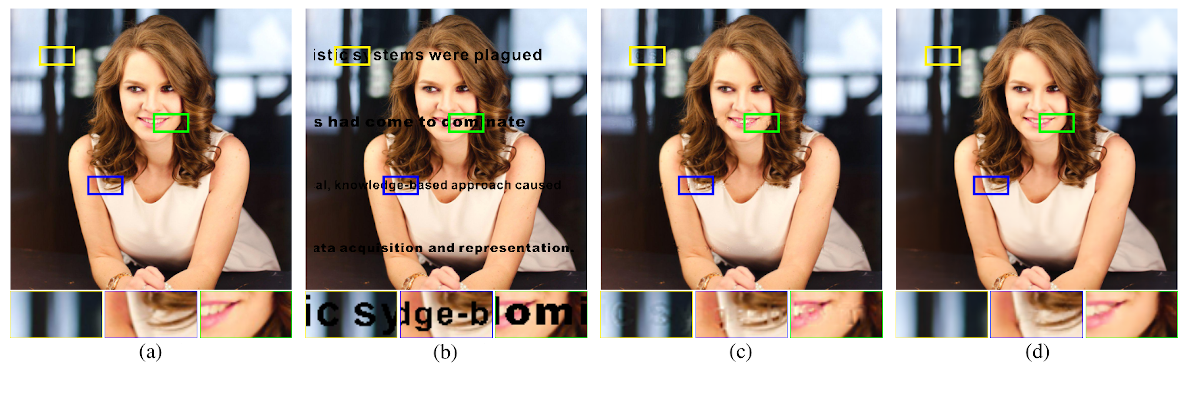
\includegraphics[width=13cm]{figures/chapter4/imprior1.png}
    \caption{Comparison between Shepard Network and Deep Image Prior \cite{shepard_nn}, \cite{deep_image_prior}}
    \label{fig:prior_shepard_comparison}
\end{figure}

In the figure \ref{fig:prior_shepard_comparison} deep image prior method compared with Shepard Neural Networks \cite{shepard_nn} which is particularly designed for inpainting applications. Using a black text as a mask, this method demonstrates astonishing results. While in the output of the Shepard network remainings of the mask can be seen, in the output of the deep image prior method there are almost no artifacts.

\begin{figure}[h]
    \centering
    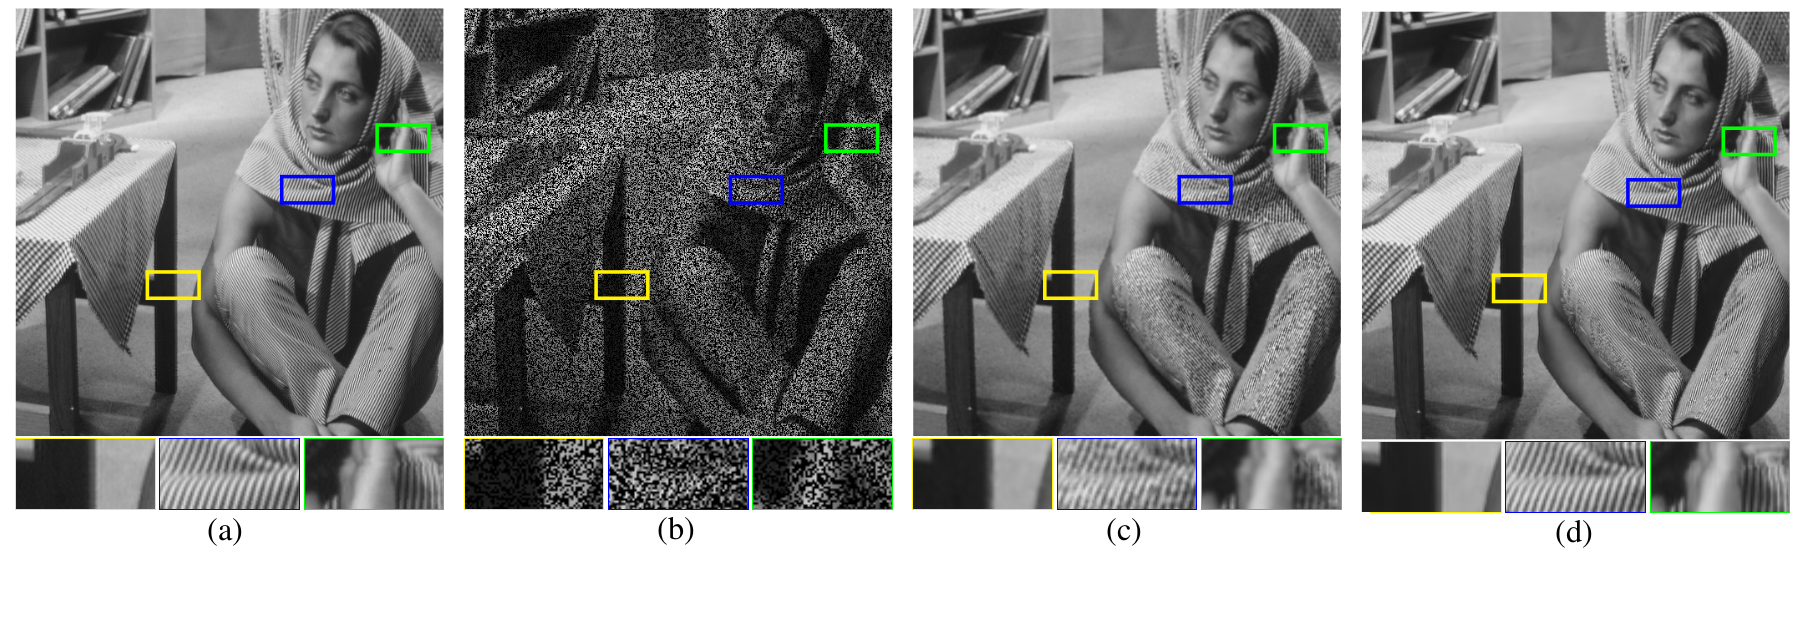
\includegraphics[width=13cm]{figures/chapter4/imprior2.png}
    \caption{Comparison between Convolutional Dictionary Learning and Deep Image Prior \cite{conv_dict_learning}, \cite{deep_image_prior}}
    \label{fig:prior_dict_camparison}
\end{figure}

In another experiment, deep image prior is compared with Convolutional Dictionary Learning method \cite{conv_dict_learning} using an image with masked half of its pixels by applying a bernoulli distrubution \cite{bernoulli} with random noise. Comparison results are given in figure \ref{fig:prior_dict_camparison}.

Apart from the inpainting study of small pixel regions, a large region inpainting process was also tested and deep image prior method has shown great success again. Although deep image prior method works great for variety of images, as a limitation it works poorly while inpainting large masked areas of the images which have highly semantic information such as face images due to being a learning-free method.

\begin{figure}[h]
    \centering
    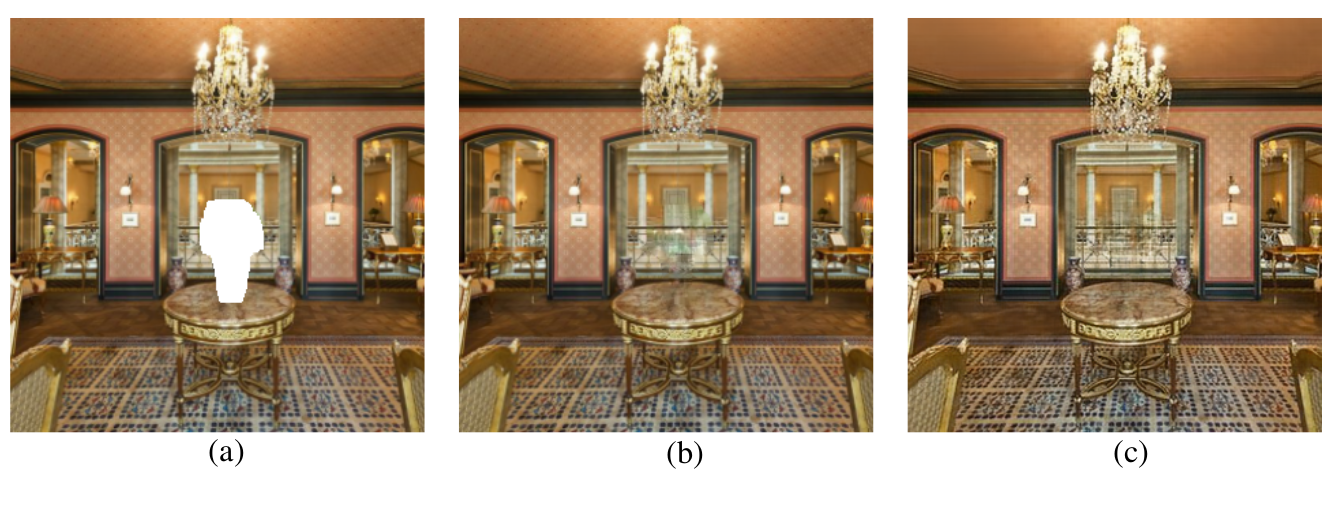
\includegraphics[width=13cm]{figures/chapter4/imprior3.png}
    \caption{Comparison between Global-Local GAN and Deep Image Prior \cite{Iizuka2017}, \cite{deep_image_prior}}
    \label{fig:prior_gan_comparison}
\end{figure}

Result of the inpainting of a large masked region with deep image prior method is compared with a learning-based generative adversarial network model \cite{Iizuka2017}. As shown in the figure \ref{fig:prior_gan_comparison}, the pretrained GAN structure performs the inpainting process with the information learned from the dataset it trained on. On the other hand deep image prior fills the missing region with texture information learned from known regions.

As mentioned, deep image prior is a method which can be applied onto any network architecture, the results obtained are highly dependent on the network structure used. In figure \ref{fig:prior_multimodels}, deep image prior method applied on different neural networks. From the results, it can be concluded that deeper networks have positive effect on the inpainting solution. However, having skip-connections which can significantly improve image recognition tasks shows extremely harmful behaviour in inpainting process as seen in figure \ref{fig:prior_multimodels}.e and \ref{fig:prior_multimodels}.f where skip-connections added to the ResNet \cite{deep_residual_recognition} and U-Net \cite{unet} architectures.

\begin{figure}[h]
    \centering
    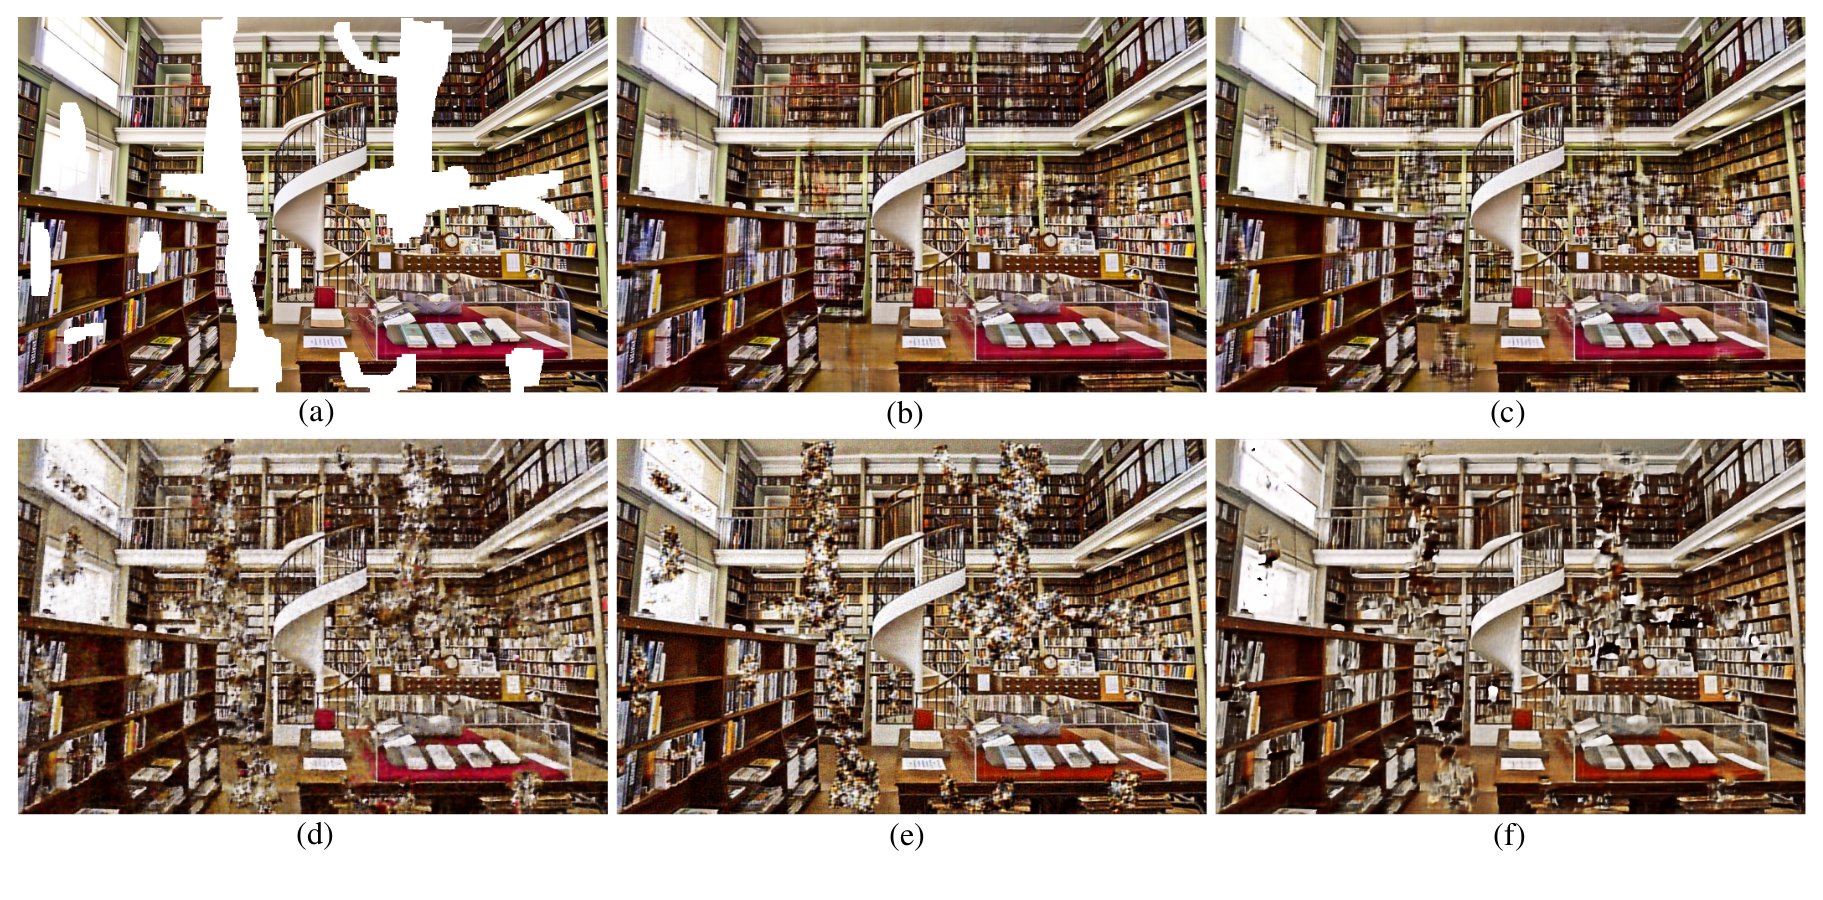
\includegraphics[width=13cm]{figures/chapter4/imprior4.png}
    \caption{Deep Image Prior results on different networks \cite{deep_image_prior}}
    \label{fig:prior_multimodels}
\end{figure}

In figures \ref{fig:prior_multimodels}.b, \ref{fig:prior_multimodels}.c and \ref{fig:prior_multimodels}.d an encoder-decoder architectures used with depth size of 6, 4, and 2 respectively. Figure \ref{fig:prior_multimodels}.e is the output of the ResNet with skip layers and with depth of 8. Figure \ref{fig:prior_multimodels}.f is the output of the U-Net structure with skip layers and depth of 5. Finally, we tested the Deep Image Prior method using a encoder-decoder network and achieved quite enough results. Figure \ref{fig:prior_lenna} shows the output of the image 512x512 image with mask we generated after 1000 iteration.

\begin{figure}[h]
    \centering
    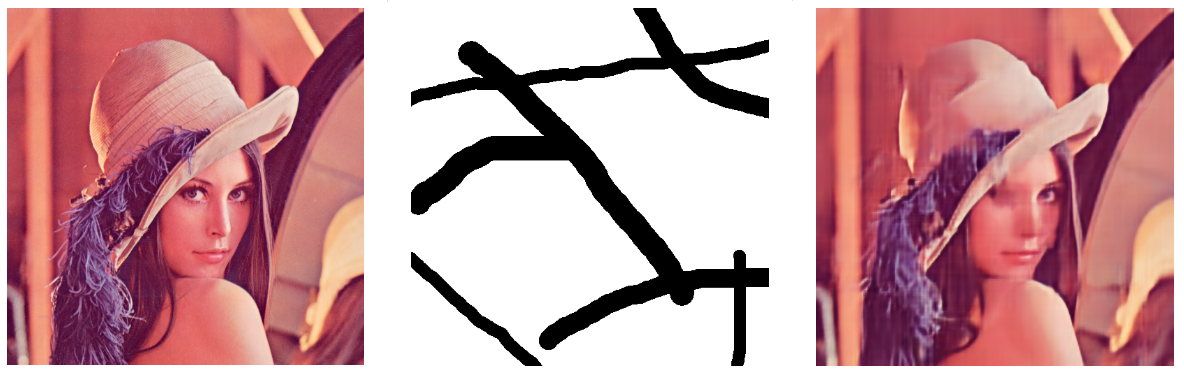
\includegraphics[width=14cm]{figures/chapter4/impriorout.png}
    \vspace*{3mm}
    \caption{Example result of the Deep Image Prior method}
    \label{fig:prior_lenna}
\end{figure}